

\documentclass{beamer}

\mode<presentation> {

% The Beamer class comes with a number of default slide themes
% which change the colors and layouts of slides. Below this is a list
% of all the themes, uncomment each in turn to see what they look like.

%\usetheme{default}
%\usetheme{AnnArbor}
%\usetheme{Antibes}
%\usetheme{Bergen}
%\usetheme{Berkeley}
%\usetheme{Berlin}
%\usetheme{Boadilla}
%\usetheme{CambridgeUS}
%\usetheme{Copenhagen}
%\usetheme{Darmstadt}
%\usetheme{Dresden}
%\usetheme{Frankfurt}
%\usetheme{Goettingen}
%\usetheme{Hannover}
%\usetheme{Ilmenau}
%\usetheme{JuanLesPins}
%\usetheme{Luebeck}
%\usetheme{Madrid}
%\usetheme{Malmoe}
%\usetheme{Marburg}
%\usetheme{Montpellier}
%\usetheme{PaloAlto}
%\usetheme{Pittsburgh}
%\usetheme{Rochester}
%\usetheme{Singapore}
%\usetheme{Szeged}
%\usetheme{Warsaw}

% As well as themes, the Beamer class has a number of color themes
% for any slide theme. Uncomment each of these in turn to see how it
% changes the colors of your current slide theme.

%\usecolortheme{albatross}
%\usecolortheme{beaver}
%\usecolortheme{beetle}
%\usecolortheme{crane}
%\usecolortheme{dolphin}
%\usecolortheme{dove}
%\usecolortheme{fly}
%\usecolortheme{lily}
%\usecolortheme{orchid}
%\usecolortheme{rose}
%\usecolortheme{seagull}
%\usecolortheme{seahorse}
%\usecolortheme{whale}
\usecolortheme{wolverine}

%\setbeamertemplate{footline} % To remove the footer line in all slides uncomment this line
%\setbeamertemplate{footline}[page number] % To replace the footer line in all slides with a simple slide count uncomment this line

%\setbeamertemplate{navigation symbols}{} % To remove the navigation symbols from the bottom of all slides uncomment this line
}

\usepackage{graphicx} % Allows including images
\usepackage{booktabs} % Allows the use of \toprule, \midrule and \bottomrule in tables


\usepackage{listings}
\lstset{language=Java,
                basicstyle=\footnotesize\ttfamily,
                keywordstyle=\footnotesize\color{blue}\ttfamily,
}

%----------------------------------------------------------------------------------------
%	TITLE PAGE
%----------------------------------------------------------------------------------------

\title[Strings]{5.Strings} % The short title appears at the bottom of every slide, the full title is only on the title page

\author{Sakib Abrar} % Your name
\institute[BUET] % Your institution as it will appear on the bottom of every slide, may be shorthand to save space
{
CSE\\~\\Bangladesh University of Engineering \& Technology \\ % Your institution for the title page
\medskip
\textit{sakib.cghs@gmail.com} % Your email address
}
\date{\today} % Date, can be changed to a custom date

\begin{document}

\begin{frame}
\titlepage % Print the title page as the first slide
\end{frame}

\begin{frame}
\frametitle{Overview} % Table of contents slide, comment this block out to remove it
\tableofcontents % Throughout your presentation, if you choose to use \section{} and \subsection{} commands, these will automatically be printed on this slide as an overview of your presentation
\end{frame}

%----------------------------------------------------------------------------------------
%	PRESENTATION SLIDES
%----------------------------------------------------------------------------------------

%------------------------------------------------
\section{String related classes}
%------------------------------------------------


\begin{frame}[fragile]{String related classes}
\begin{itemize}
\item Java provides three String related classes
\item java.lang package\\
–String class: Storing and processing Strings but Strings
created using the String class cannot be modified
immutable\\
–StringBuffer class: Create flexible Strings that can be
modified\\
\item java.util package\\
–StringTokenizer class: Can be used to extract tokens from a
String
\end{itemize}
\end{frame}

%------------------------------------------------
\section{String basics}
%------------------------------------------------

\begin{frame}
\frametitle{String Basics}
\begin{itemize}
\item String class provide many constructors and more
than 40 methods for examining in individual
characters in a sequence.\\
\item You can create a String from a String value or from an
array of characters.\\
–String newString = new String(stringValue);\\
\item The argument stringValue is a sequence of characters
enclosed inside double quotes\\
–String message = new String (“Welcome”);\\
–String message = “Welcome”;
\end{itemize}
\end{frame}


%------------------------------------------------
\section{String constructors}
%------------------------------------------------

\begin{frame}
\frametitle{String constructors}
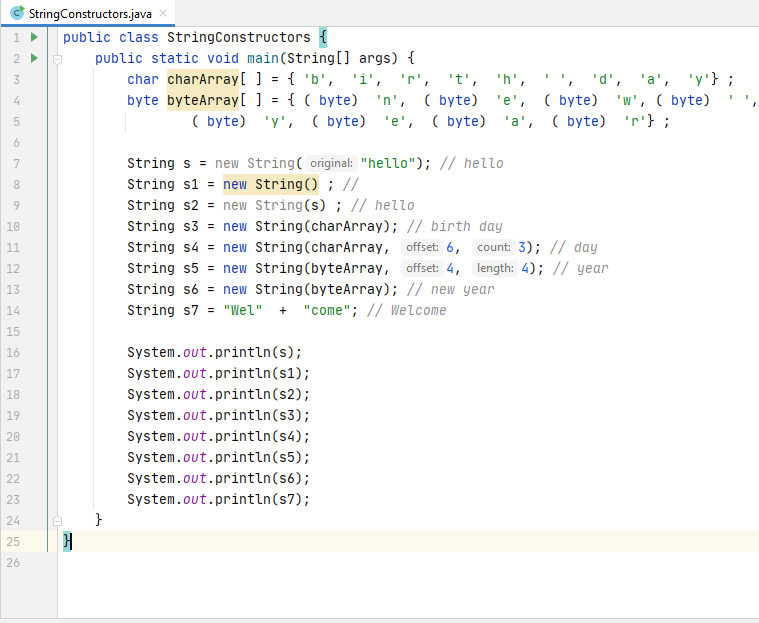
\includegraphics[width=0.9\textwidth]{StringConstructors.png}
\end{frame}



%-----------------------------------------------
\section{String length and character extraction}
%-----------------------------------------------

\begin{frame}{String length \& character extraction}
\begin{itemize}
\item Returns the length of a String\\
–length()\\
\item Example:\\
String s1=“Hello”; \\
System.out.println(s1.length);
\end{itemize}

\textbf{Extraction}
\begin{itemize}
\item Get the character at a specific location in a string\\
–s1.charAt(1)
\item Get the entire set of characters in a string\\
–s1.getChars(0, 5, charArray, 0)
\end{itemize}

\end{frame}


%-----------------------------------------------
\section{Extracting Substrings}
%------------------------------------------------

\begin{frame}[fragile]
\frametitle{Extracting Substrings}
\begin{itemize}
\item substring method enable a new String object to be
created by copying part of an existing String object\\
–substring (int startIndex) ‐ copies the characters form the
starting index to the end of the String\\
–substring(int beginIndex, int endIndex) ‐ copies the
characters from the starting index to one beyond the
endIndex\\
\end{itemize}
\end{frame}

%------------------------------------------------

%-----------------------------------------------
\section{String Comparisons}
%------------------------------------------------

\begin{frame}
\frametitle{String Comparisons}
\begin{itemize}
\item equals\\
–Compare any two string objects for equality using
lexicographical comparison. s1.equals(“hello”)
\item equalsIgnoreCase\\
–s1.equalsIgnoreCase(s2)
\item compareTo\\
–s1.compareTo(s2)\\
–s1 > s2 (positive), s1 < s2 (negative), s1 = s2 (zero)
\end{itemize}
\end{frame}

%------------------------------------------------


%-----------------------------------------------
\section{String Concatenation}
%------------------------------------------------

\begin{frame}
\frametitle{String Concatenation}
\begin{itemize}
\item Java provide the concat method to concatenate two
strings.\\
String s1 = new String (“Happy ”);\\
String s2 = new String (“Birthday”);\\
String s3 = s1.concat(s2);\\
s3 will be “Happy Birthday”\\
\end{itemize}


\end{frame}

%------------------------------------------------

%-----------------------------------------------
\section{String Search}
%------------------------------------------------

\begin{frame}
\frametitle{String Search}
\begin{itemize}
\item Find the position of character/String within a String\\
–int indexOf (char ch)\\
–int lastIndexOf (char ch)\\
\end{itemize}
\end{frame}

%------------------------------------------------

%-----------------------------------------------
\section{String Split}
%------------------------------------------------

\begin{frame}
\frametitle{String Split}
\begin{itemize}
\item split() method splits a String against given regular
expression and returns a character array
\item String test = "abc,def,123";\\
String[] out = test.split(",");\\
out[0] - abc , out[1] - def, out[2] - 123
\end{itemize}
\end{frame}

%------------------------------------------------

%-----------------------------------------------
\section{String Conversions}
%------------------------------------------------

\begin{frame}
\frametitle{String Conversions}
\begin{itemize}
\item Generally, the contents of a String cannot be
changed once the string is created,
\item Java provides conversion methods
\item \textbf{toUpperCase()} and \textbf{toLowerCase()}\\
–Converts all the characters in the string to lowercase or
uppercase\\
\item \textbf{trim()}\\
–Eliminates blank characters from both ends of the string\\
\item \textbf{replace(oldChar, newChar)}\\
–Replaces a character in the string with a new character
\end{itemize}
\end{frame}

%------------------------------------------------


%-----------------------------------------------
\section{String to other type conversions}
%------------------------------------------------

\begin{frame}
\frametitle{String to other type conversions}
The String class provides \textbf{valueOf} methods for
converting a character, an array of characters and
numeric values to strings\\
–\textbf{valueOf} method take different argument types\\~\\
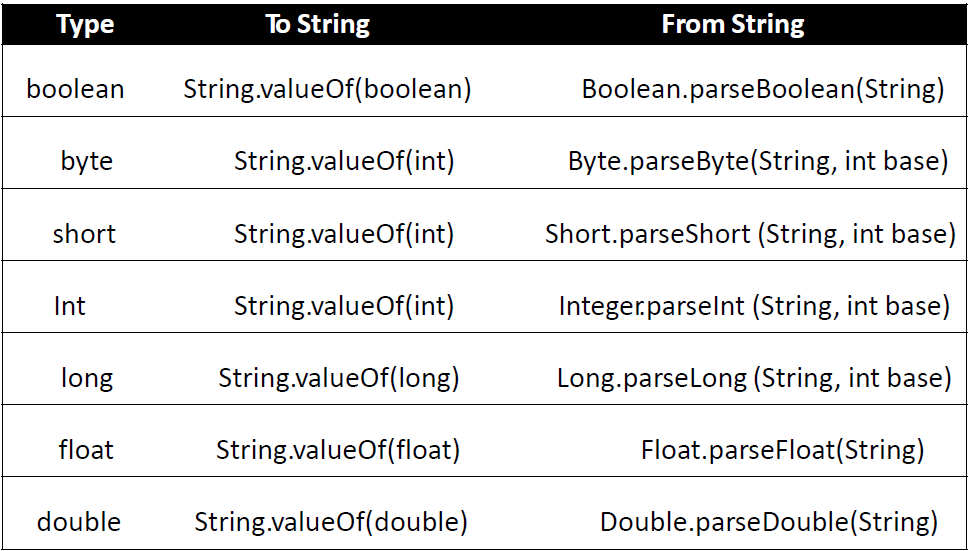
\includegraphics[width=0.95\textwidth]{valueOf.png}
\end{frame}

%------------------------------------------------


%--------------------------------------------------

\begin{frame}
\Huge{\centerline{THE END }}
\end{frame}

%----------------------------------------------------------------------------------------

\end{document} 